\documentclass{ibetest}
\begin{document}
\maketest{Progress Test 1.B --- Thermo-S1}
         {1.B \,$\cdot$\, Postulates of thermodynamics}
         {7 minutes}{14}

% ---------------------------------------------------------------------------
\exercise{Temperature conversion}{1 mark}
Liquid nitrogen boils at $T = \qty{77}{K}$ under atmospheric pressure. Express this
temperature in degrees Celsius, exactly.
\answer{1}{2.2cm}{%
  $\theta = T - 273.15 = 77 - 273.15$ \qquad $\boxed{\theta = -196.15\ ^\circ\mathrm C}$}
\begin{scheme}
\pt{1}{1 pt}{$-196.15\ ^\circ$C (the minus sign is part of the answer).}
\end{scheme}
\begin{tip}
The kelvin is written with a capital K and no degree sign: ``77 K'', not ``77\,$^\circ$K''.
Test~1's marker noted: ``big K stands for kelvins''.
\end{tip}

% ---------------------------------------------------------------------------
\exercise{Thermodynamic equilibrium --- postulates}{5 marks}
A system is in contact with surroundings at pressure $p_0$ and temperature $T_0$. Give the two
conditions of thermodynamic equilibrium, with the corresponding equalities. State the
postulates of classical thermodynamics. When are the state variables of a system defined?
\answer{2,2,1}{6.2cm}{%
  \textbf{Thermal equilibrium:} $T_{\text{system}} = T_0$.\quad
  \textbf{Mechanical equilibrium:} $p_{\text{system}} = p_0$ (for a movable wall).\\[4pt]
  \textbf{Postulates.}\\
  (1) A system left to itself (isolated, or in constant surroundings) evolves spontaneously
  towards an equilibrium state, and then no longer leaves it.\\
  (2) At equilibrium, the state of the system is completely described by a
  \emph{small number} of macroscopic state variables ($p$, $V$, $T$, $n$). There is no need
  for the positions and velocities of all the particles.\\[4pt]
  The state variables are defined (uniform in space and constant in time) \textbf{only at
  equilibrium}. Between two equilibrium states they may not be defined.}
\begin{scheme}
\pt{1}{2 pts}{$T = T_0$ (thermal) and $p = p_0$ (mechanical), 1~pt each.}
\pt{2}{2 pts}{Evolution towards equilibrium (1~pt); a few state variables suffice (1~pt).}
\pt{3}{1 pt}{State variables are defined only at equilibrium.}
\end{scheme}
\begin{note}
Box~8 is blank in the handout. These are the standard statements; accept the wording given
in class.
\end{note}

% ---------------------------------------------------------------------------
\exercise{Equilibrium or not?}{4 marks}
\question{A syringe with a free, sealed piston is left for a long time in a room at
  $(p_0, T_0)$. The enclosed gas then has:}
\opttwo{1}{$p = p_0$ and $T = T_0$}{0}{$p > p_0$ and $T = T_0$}
       {0}{$p = p_0$ and $T > T_0$}{0}{$p$ and $T$ not defined}
\why{once equilibrium is reached, the state variables of the system equal those of the
  surroundings (Fig.~3 and remark~(i)).}
\question{Just after a sudden push on the piston, the pressure of the gas:}
\opttwo{0}{already has its final value}{1}{is not defined: it is not uniform}
       {0}{is equal to $p_0$}{0}{is zero}
\why{it takes some time for $p$ and $T$ to become uniform and steady again: state variables
  exist only at equilibrium.}
\question{A metal rod has one end in boiling water and the other in melting ice. Its
  temperature profile no longer changes. The rod is:}
\opttwo{0}{at thermodynamic equilibrium}{1}{in a steady state, not at equilibrium}
       {0}{isolated}{0}{at equilibrium: nothing changes}
\why{equilibrium requires \emph{both} a steady state and homogeneity. Here $T$ varies along
  the rod.}
\question{To describe a closed system at equilibrium, classical thermodynamics uses:}
\opttwo{0}{all positions and velocities}{1}{a few state variables ($p$, $V$, $T$)}
       {0}{only its mass}{0}{its whole past history}
\why{this is the second postulate (remark~(ii) of the notes).}

% ---------------------------------------------------------------------------
\exercise{A loaded piston}{4 marks}
\noindent\begin{minipage}[c]{0.6\textwidth}
A vertical cylinder is closed by a frictionless piston of area $S$ and negligible mass. The
surroundings are at $p_0$ and $T_0$. A mass $m$ is placed on the piston. Find the pressure and
the temperature of the gas once equilibrium is reached.
\end{minipage}\hfill
\begin{minipage}[c]{0.36\textwidth}\centering
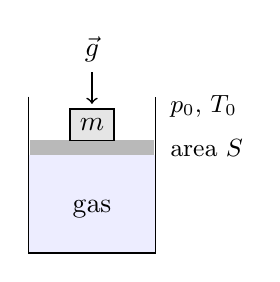
\begin{tikzpicture}[scale=0.62, line width=0.6pt]
  \fill[blue!7] (0,0) rectangle (2.6,2.0);
  \draw (0,3.2) -- (0,0) -- (2.6,0) -- (2.6,3.2);
  \node at (1.3,0.9) {gas};
  \fill[gray!55] (0.03,2.0) rectangle (2.57,2.3);
  \draw[fill=gray!20] (0.85,2.3) rectangle (1.75,2.95); \node at (1.3,2.62) {$m$};
  \draw[->] (1.3,3.7) -- (1.3,3.05) node[pos=0, above] {$\vec g$};
  \node[right, font=\small] at (2.7,2.15) {area $S$};
  \node[right, font=\small] at (2.7,3.0) {$p_0$, $T_0$};
\end{tikzpicture}
\end{minipage}
\data{$p_0 = \qty{1.0e5}{Pa}$ \hspace{12mm} $T_0 = \qty{293}{K}$ \hspace{12mm}
      $m = \qty{1.0}{kg}$\\[2pt]
      $S = \qty{2.0}{\centi\metre\squared}$ \hspace{12mm} $g = \qty{10}{\metre\per\second\squared}$}
\answer{1,1,1,1}{5.8cm}{%
  Equilibrium of the piston: $pS = p_0S + mg$ \quad$\Rightarrow$\quad
  $\boxed{p = p_0 + \dfrac{mg}{S}}$\\[4pt]
  $S = 2.0\ \mathrm{cm^2} = 2.0\times(10^{-2}\ \mathrm m)^2 = 2.0\times10^{-4}\ \mathrm{m^2}$
  \qquad $\dfrac{mg}{S} = \dfrac{1.0\times10}{2.0\times10^{-4}}\ \mathrm{Pa}
  = 5.0\times10^{4}\ \mathrm{Pa}$\\[4pt]
  $\boxed{p = 1.5\times10^{5}\ \mathrm{Pa}}$ \qquad and, once thermal equilibrium is
  reached, \quad $\boxed{T = T_0 = 293\ \mathrm K}$}
\begin{scheme}
\pt{1}{1 pt}{Force balance on the piston: $p = p_0 + mg/S$ (literal).}
\pt{2}{1 pt}{$S = 2.0\times10^{-4}\ \mathrm{m^2}$.}
\pt{3}{1 pt}{$p = 1.5\times10^{5}\ \mathrm{Pa}$.}
\pt{4}{1 pt}{$T = T_0 = 293\ \mathrm K$ (thermal equilibrium).}
\end{scheme}
\begin{tip}
$1\ \mathrm{cm^2} = (10^{-2}\ \mathrm m)^2 = 10^{-4}\ \mathrm{m^2}$, not $10^{-2}$. As in
Test~1: keep letters until the end, then substitute with units.
\end{tip}

\finish
\end{document}
